\section{Project Description} \label{sec:project_description}
The objective of this project was to implement a 16-bit Kogge-Stone Adder in \SI{0.35}{\micro\m} technology which from now on will be called KS adder. The KS adder belongs to the family of parallel-prefix adders which reduces the critical path compared to regular ripple-carry adders. The cost for this is paid in area and complex routing which prolongs development time.

Fast adders are very important in all types of integrated circuits since almost all algorithms one can come up with consists of at least one one addition. 

The official goal was to reach a speed of \SI{200}{\mega\Hz} but the group decided on an unofficial goal to reach a speed of \SI{400}{\mega\Hz}.

\begin{figure}[H]
  \centering
  \captionsetup{justification=centering}
  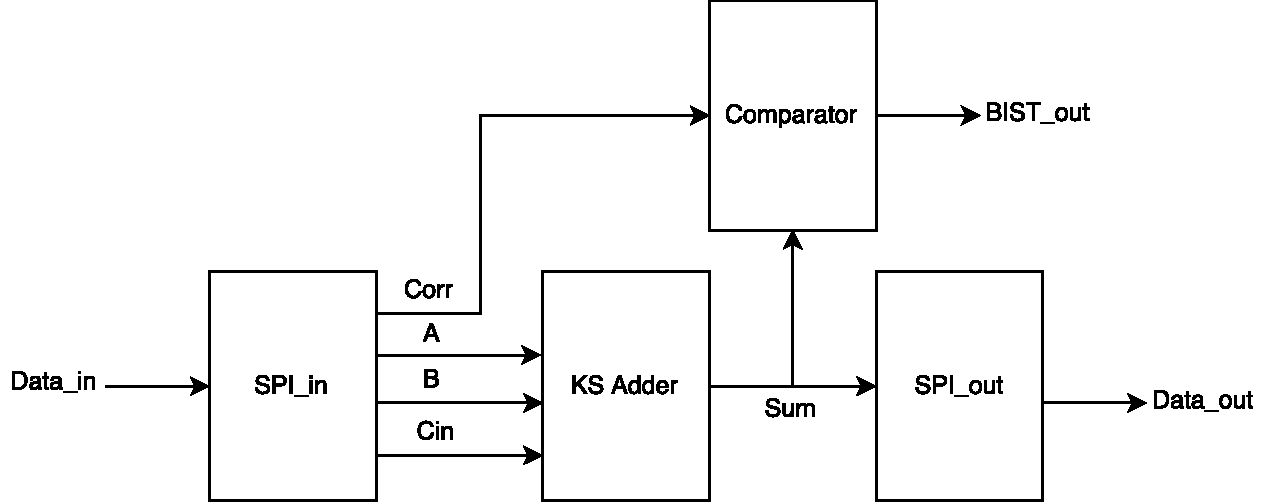
\includegraphics[scale=0.5]{../figures/TOP.pdf}
  \caption{Block diagram of the system first iteration.} \label{fig:block_first}
\end{figure}

\begin{figure}[H]
\centering
\captionsetup{justification=centering}
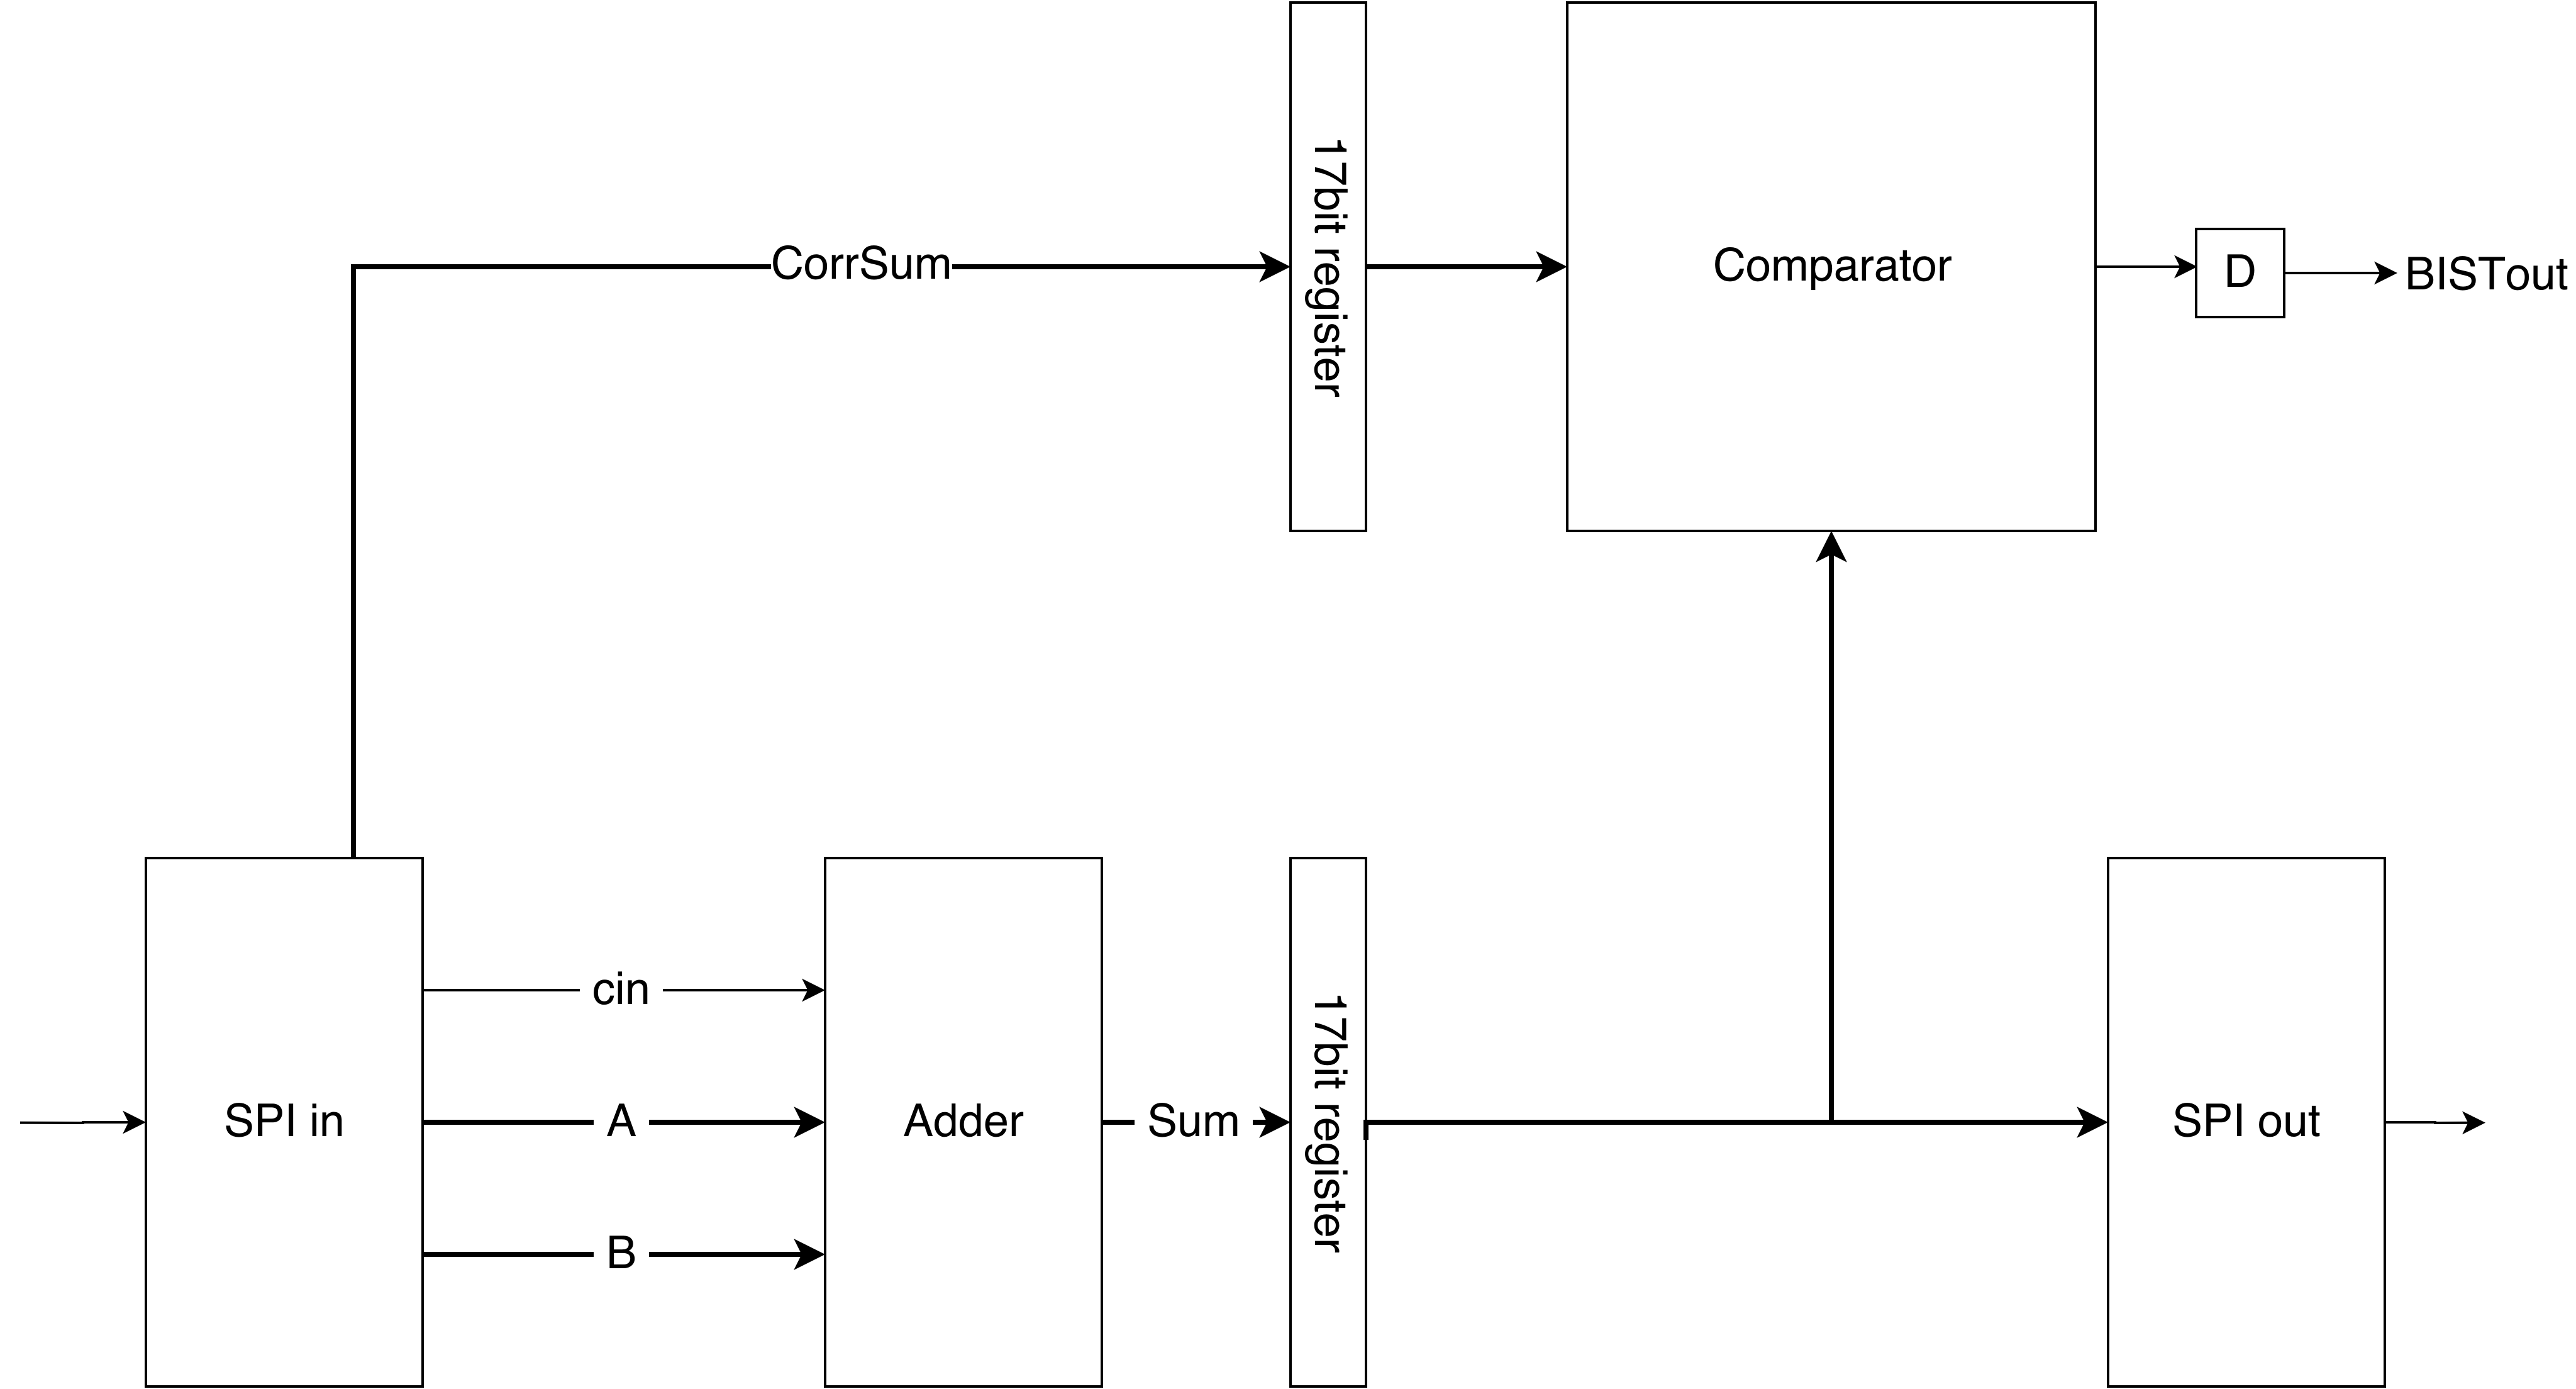
\includegraphics[scale=0.1]{../figures/top_level_second.png}
\caption{Block diagram of the system second iteration.} \label{fig:block_second}
\end{figure}

\begin{figure}[H]
\centering
\captionsetup{justification=centering}
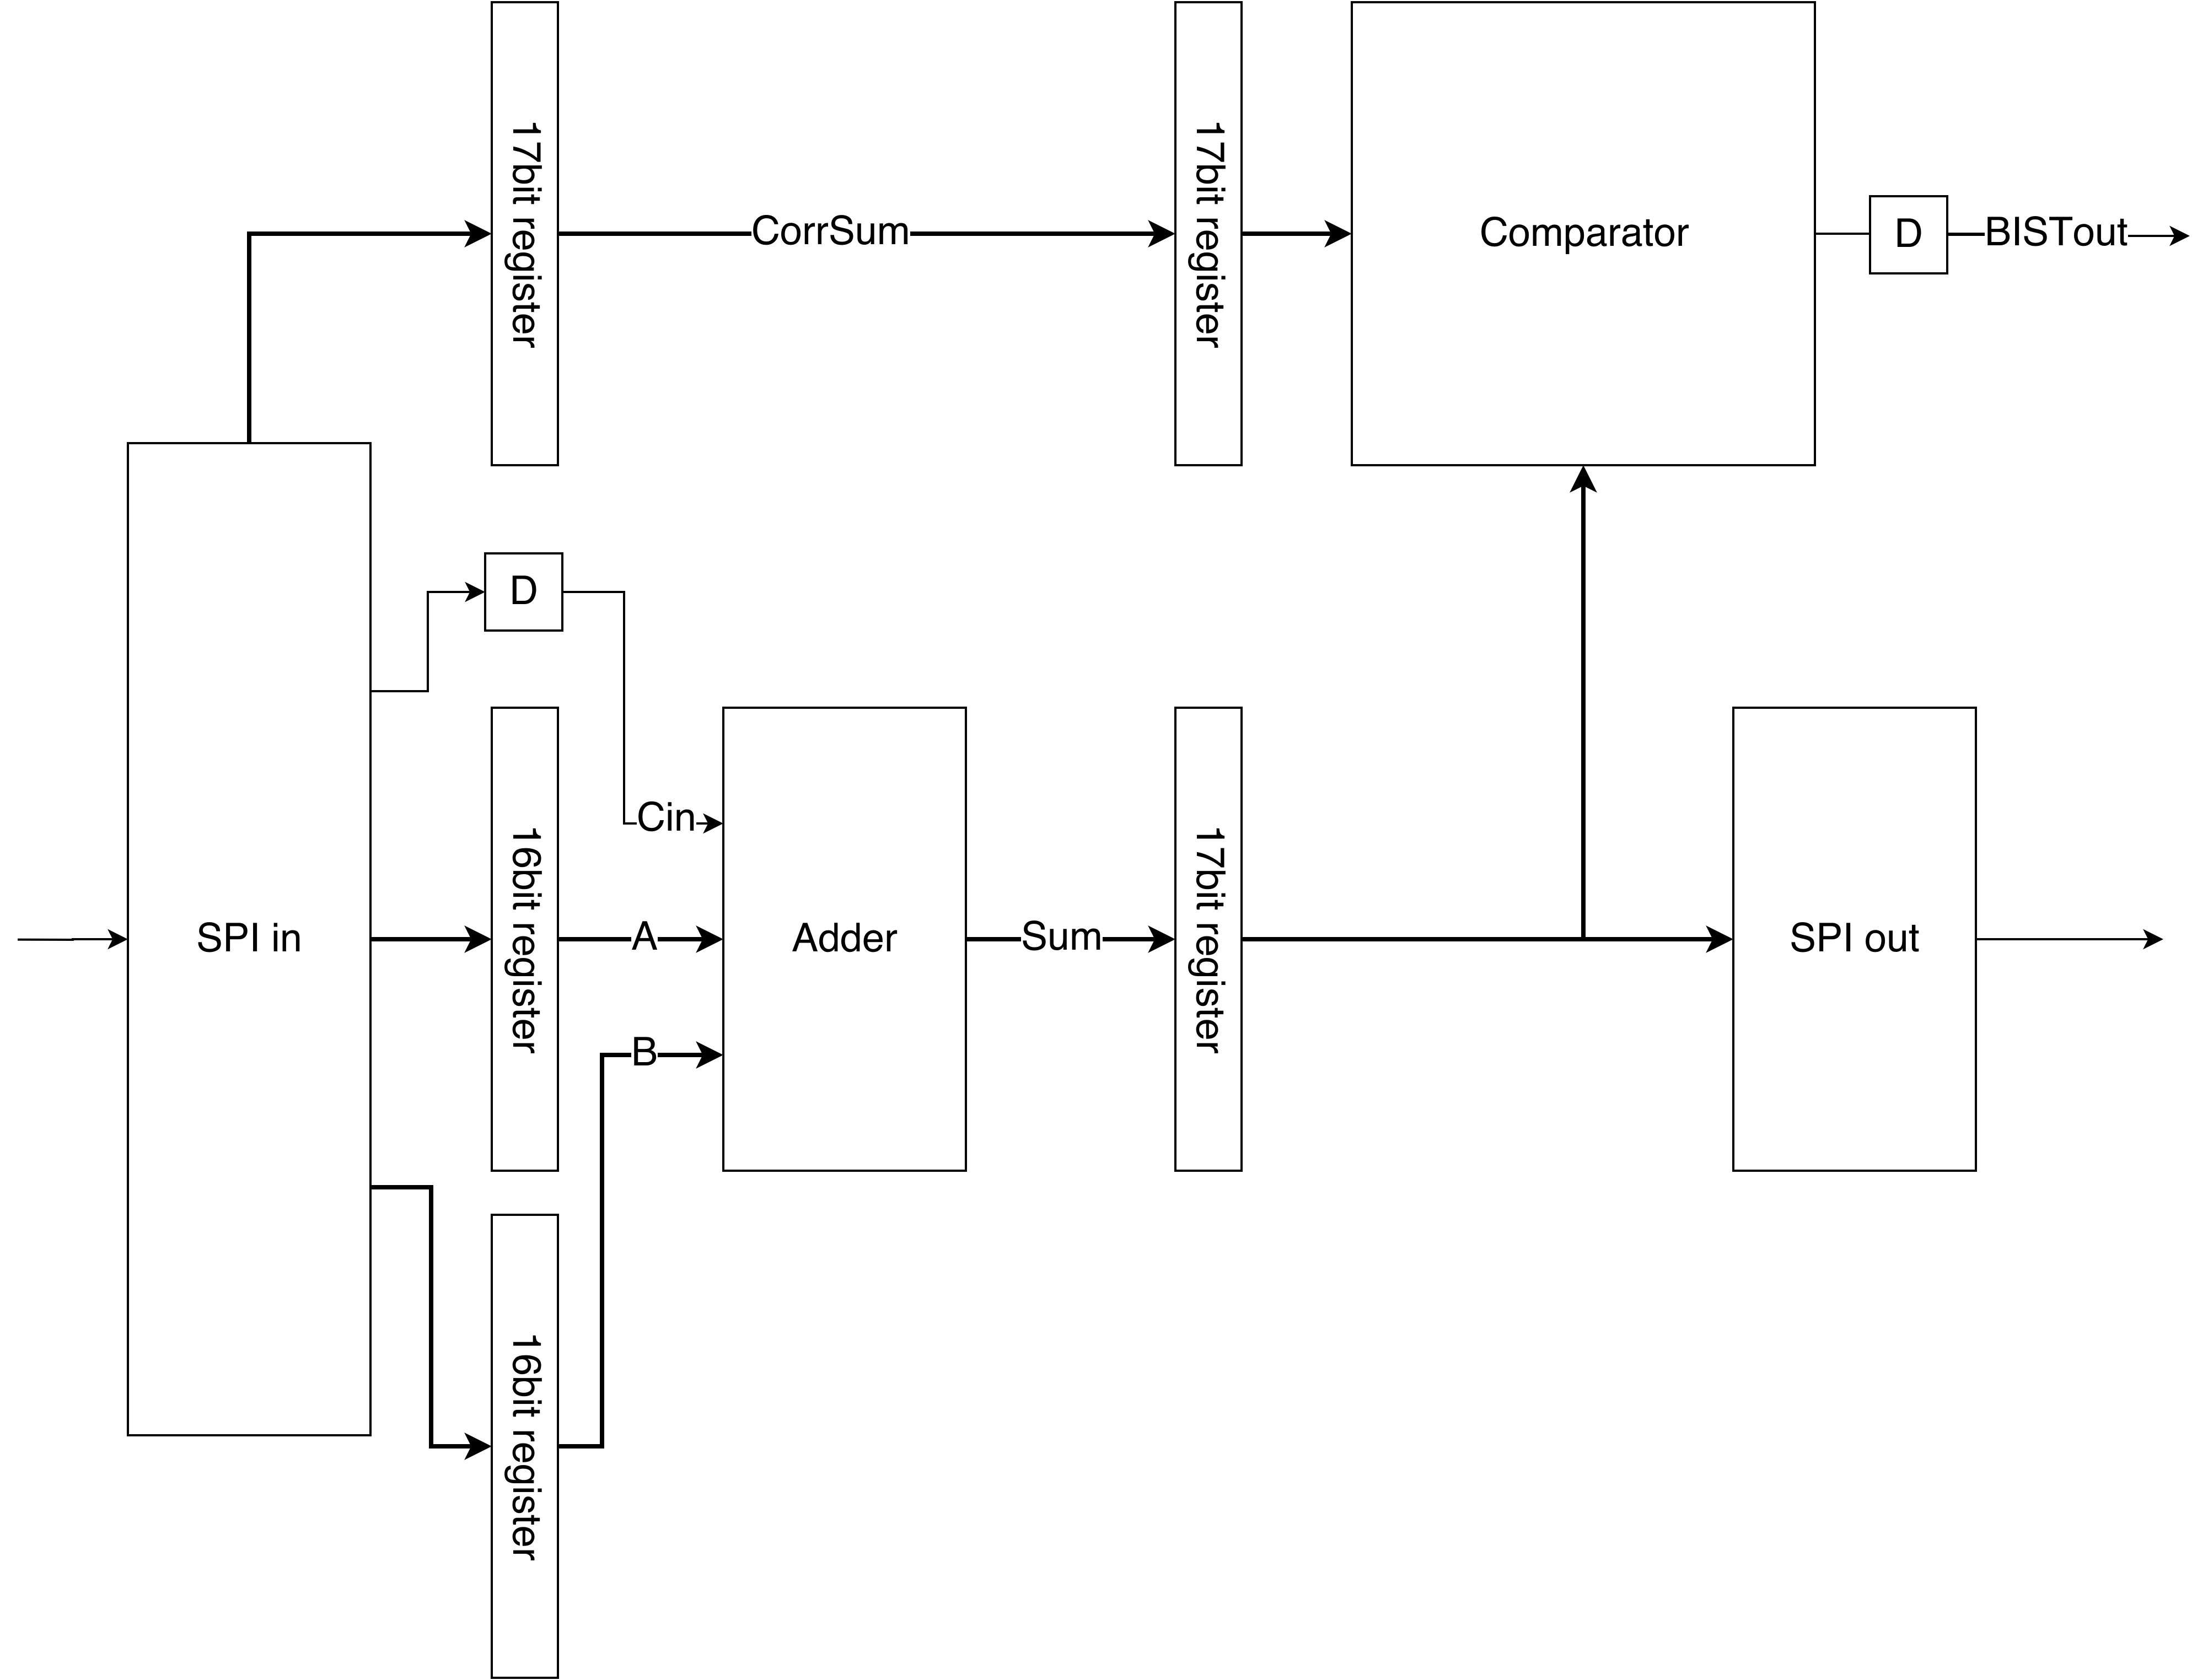
\includegraphics[scale=0.1]{../figures/top_level_final.png}
\caption{Block diagram of the system final iteration.}  \label{fig:block_final}
\end{figure}

In Figure \ref{fig:block_first} the block diagram of the system after the first design phase is depicted. One can note that the signal goes from one block to the next directly. In figure \ref{fig:block_second} some registers have been introduced to make sure BISTout stays the same between clock pulses when new data is evaluated and to give a more stable signal to the comparator and SPI-out unit. In the final iteration additional register have been inserted between SPI in and the adder to cut the path from the registers in the SPI unit to the adder and to make sure that all bits in the same word arrives at the same time to the adder. The block diagram from the last iteration can be seen in Figure \ref{fig:block_final}.
